We begin by expanding the mismatch summation from equation~\eqref{eqn: mismatch}.
Writing the summations explicitly we have
\begin{align}
m & = g_{\alpha\beta i j}\dl^{\alpha i}\dl^{\beta j}  \\
&=\s{i=1}{N}\s{j=1}{N}g_{\alpha\beta i j}\dl^{\alpha i}\dl^{\beta j}  \\
&= \s{i=1}{N}g_{\alpha\beta i i}\dl^{\alpha i}\dl^{\beta i} 
+ \s{i=1}{N} \s{\substack{j=1\\ j \ne i}}{N} g_{\alpha \beta ij}\dl^{\alpha i}\dl^{\beta j}  
\end{align}
The summation has been intentionally split into terms for which the two segments
are the same and those where they are different. The metric when the reference
time is at the beginning of each segment is given by equation 
\eqref{eqn: metric equal segments tref 0}. By considering the metric for the two cases we can write
the two distinct components as
\begin{equation}
g_{\alpha\beta ij} = \left\{
\begin{array}{cc}
g_{\alpha\beta}^{E} & \textrm{ if } i =j \\
g_{\alpha\beta}^{NE} & \textrm{ if } i  \ne j 
\end{array}•\right. 
\end{equation}
The mismatch is then given by computing
\begin{align}
m &= \s{i=1}{N}g_{\alpha\beta}^{E}\dl^{\alpha i}\dl^{\beta i} 
+ 2\s{i=1}{N} \s{j=1}{i-1} g_{\alpha \beta}^{NE}\dl^{\alpha i}\dl^{\beta j} 
\label{eqn: mismatch sep}
\end{align}

\subsubsection{Writing the parameter offsets in terms of normal distributions}
Equations \eqref{eqn: fdot offset}, \eqref{eqn: f offset}, and \eqref{eqn: phi
offset} give the offsets as functions of the offsets in higher order
parameters. In order to calculate statistical values we write these in terms of
the normal distributions from which the random walks are constructed. Substituting \eqref{eqn: fdot
offset} into \eqref{eqn: f offset} and using the summation properties defined
in appendix \ref{sec: summation identities} we have
\begin{align}
\Delta \f_{i}  & = \s{j=1}{i}\tn \f_{j} 
+ \s{j=1}{i-1}\s{k=1}{j}\tn \fdot_{k} \dT ,  \\
& = \s{j=1}{i}\tn \f_{j} 
+ \s{j=1}{i-1}(i-j)\tn \fdot_{j} \dT . \label{eqn: f hat offset}
\end{align}
Similarly substituting this equation into equation~\eqref{eqn: phi offset} we
have
\begin{align}
\Delta\phi_{i} & = \s{j=1}{i}\tn \phi_{j} 
+ 2\pi \left(\s{j=1}{i-1}\Delta\f_{j}\dT 
+ \frac{1}{2}\s{j=1}{i-1}\Delta\fdot_{j}\dT^{2}\right) \notag \\
& = \s{j=1}{i}\tn \phi_{j} + 2\pi\left(\s{j=1}{i-1}\left(\s{k=1}{j}\tn\f_{k} 
+ \s{k=1}{j-1}(j-k)\tn\fdot_{k}\dT\right)\dT
 + \frac{1}{2}\s{j=1}{i-1}\s{k=1}{j}\Delta\fdot_{k}\dT^{2} \right)  \notag \\
& = \s{j=1}{i}\tn \phi_{j} + 2\pi\left(\s{j=1}{i-1}(i-j)\tn\f_{j}\dT
 + \s{j=1}{i-1}\s{k=1}{j-1}(j-k)\tn\fdot_{k}\dT^{2}
 + \frac{1}{2}\s{j=1}{i-1}(i-j)\Delta\fdot_{j}\dT^{2} \right)  \notag \\
& = \s{j=1}{i}\tn \phi_{j} + 2\pi\left(\s{j=1}{i-1}(i-j)\tn\f_{j}\dT 
 + \frac{1}{2}\s{j=1}{i-1}\left(\left(i-j\right)\left(i-j-1)\right) 
 + (i-j)\right)\tn\fdot_{j}\dT^{2}\right)  \notag\\
& = \s{j=1}{i}\tn \phi_{j} + 2\pi\left(\s{j=1}{i-1}(i-j)\tn\f_{j}\dT 
 + \frac{1}{2}\s{j=1}{i-1}(i-j)^{2}\tn\fdot_{j}\dT^{2}\right)  \notag\\
\end{align}

All the parameter space offsets are know written purely in terms of the 
distributions $\tn \phi_i$, $\tn \f_i$, and $\tn \fdot_i$. 
%
\subsubsection{Distribution of jumps}
In equation~\eqref{eqn: fdot offset}  we defined the steps in spin-down to be
normally distributed. Therefore the jumps between spin-down values will also be
normally distributed, that is $\fdot_{i} - \fdot_{i-1} \sim N(0, \sigS)$. In
the lower order terms, for example the frequency, we can have a mix of the
random walk in frequency and the induced effect of the random walk in spin-down;
the same is true for the phase but with an induced effect from the frequency
and spin-down.  We now investigate how the induced effect of higher order random
walks effects on the distributed of jumps in frequency and phase. To check this
we  look at the distribution at the $i^{th}$ step using equation 
\eqref{eqn: f hat offset}
\begin{align}
\Delta \f_{i} - \Delta \f_{i-1} & = \s{j=1}{i}\tn \f_{j}
-  \s{j=1}{i-1}\tn \f_{j} + \left(\s{j=1}{i-1}(i-j)\tn \fdot_{j}  
-  \s{j=1}{i-2}(i-1-j)\tn \fdot_{k} \right)\dT  \\
& = \tn \f_{i} + \left(\tn \fdot_{i-1} 
+ \s{j=1}{i-2}(i-j-i+1+j)\tn \fdot_{j}\right)\dT \\
& = \tn \f_{i} + \s{j=1}{i-1}\tn \fdot_{j} \dT \\
& \sim N(0, \sigF) + \s{j=1}{i-1}N(0, \sigS) \dT 
\end{align}
To combine the distributions we use the summation property of normal
distributions. For a central normal distribution $X_{i}\sim N(0,
\sigma_{i}^{2})$, the sum of $N$ terms with real coefficients $a_{i}$ is given
by 
\begin{equation}
\s{i=1}{N}a_{i}X_{i} \sim N\left(0, \s{i=1}{N}(a_{i}\sigma_{i})^{2}\right).
\end{equation}
Then we have
\begin{align}
\Delta \f_{i} - \Delta \f_{i-1} & \sim N(0, \sigF) 
+ N\left(0, \s{j=1}{i-1}(\sigS\dT)^{2}\right) \\
& \sim N(0, \sigF) + N(0, (i-1)\sigS\dT^{2}) \\
& \sim N(0, \sigF + (i-1)\sigS\dT^2)  
\end{align}
Similarly for the phase 
\begin{align}
\Delta \phi_{i} - \Delta \phi_{i-1} = &  \left(\s{j=1}{i}\tn \phi_{j} 
-  \s{j=1}{i-1}\tn \phi_{j}\right) + 2\pi\left(\s{j=1}{i-1}(i-j)\tn \f_{j}  
-  \s{j=1}{i-2}(i-1-j)\tn \f_{k} \right)\dT \notag \\
& + \pi\left(\s{j=1}{i-1}(i-j)^{2}\tn \fdot_{j} 
- \s{j=1}{i-2}(i-1-j)^{2}\tn \fdot_{j}\right)\dT^{2} \\
= &  \tn \phi_{i} +  2\pi \s{j=1}{i-1}\tn\f_{j} 
+ \pi \s{j=1}{i-1}(2i - 2j -1)\fdot_{j}\dT^{2} \\
\sim &  N(0, \sigS) + \s{j=1}{i-1}N(0, \sigF) \dT 
+ \s{j=1}{i-1}(2i - 2j -1)N(0, \sigS) \dT^{2}  \\
\sim &  N\left(0, \sigS\right) + N\left(0, (i-1)\sigF\dT^{2}\right) 
+ N\left(0, \s{j=1}{i-1}(2i - 2j -1)\sigS\dT^{4}\right)  \\
\sim &  N\left(0, \sigS\right) + N\left(0, (i-1)\sigF\dT^{2}\right) 
+ N\left(0, (i-1)^{2}\sigS\dT^{4}\right)  \\
\Delta \phi_{i} - \Delta \phi_{i-1}  \sim & N\left(0, \sigS 
+ (i-1)\sigF\dT^{2} + (i-1)^{2}\sigS\dT^{4}\right)
\end{align}

This result indicates that the integrated effect of random walks in higher
order terms will create a normal distribution in the monthly ephemeris. The
standard deviation will
depend on the observation time. 

\paragraph{Taking the expectation}
To infer the behaviour of the mismatch under this random walk we will take the
expectation of equation~\eqref{eqn: mismatch sep} having inserted the
expressions for the parameter offsets written in terms of normal distributions.
This will yield a number of terms with all the permutations of two terms from
$[\tn \phi, \tn \f, \tn \fdot]$. All the cross-correlated terms such as
$\tn\phi_{i}\tn \fdot$ will have an expectation of zero since the steps of the
random walk are independent. The only non-vanishing terms are given by
\begin{align}
E[\tn\phi_{i}\tn\phi_{j}] &= \delta_{ij}\sigP, & 
E[\tn\f_{i}\tn\f_{j}] &= \delta_{ij}\sigF,& 
E[\tn\fdot_{i}\tn\fdot_{j}] &= \delta_{ij}\sigS, 
\end{align}
Inserting these expression into equation~\eqref{eqn: mismatch sep} 
we find the mismatch is given by
\begin{align}
E[m]   = &  \frac{A_{\phi}}{6} \left(N - \frac{1}{N}\right) 
+ \frac{\pi^{2} A_{{f}}}{30}\left(4 N^{3} + 5 N^{2} + \frac{1}{N}\right)\\
 & +  \frac{\pi^{2} A_{{\dot{f}}}}{3780} \left(66 N^{5} - 21 N^{3} + 105 N^{2} 
 + 217 N + 63 - \frac{94}{N}\right)
\label{eqn: expectation}
\end{align}•
where 
\begin{equation}
	A_{\phi} = \sigP \;\;\;\;\; 
    A_{\f} = \sigF\Delta T^{2} \;\;\;\;\; 
    A_{\fdot} = \sigF\Delta T^{4}.
\end{equation}

\paragraph{Implied scaling}
Equation~\eqref{eqn: expectation} predicts the variation in mismatch with
observation time due to a random walk in the parameters of the signal. The
random walk occurs at fixed intervals of $\dT$ and in three parameters, as such
the mismatch is a function of all these variables. This method differs from
results in the literature studying timing noise \citep{Cordes1981} where the
steps are Poisson distributed in time with an average rate. The choice of a
fixed $\dT$ is motivated by results from the Crab ephemeris in which the
segment duration is fixed at 1 month. For the expectation of the mismatch to be
physical, we should expect that, at least to leading order, it
is invariant to a suitable combination of $\dT$ and $\sigma$.  Equivalently we
imagine that if the Crab ephemeris was updated every half a month, we
should measure the same mismatch for the same observation period. 

To leading order, for the expected mismatch to be invariant to changes in $\dT$
we require
\begin{equation}
\sigP \sim \dT \;\;\;\;\; \sigF \sim \dT \;\;\;\;\; \sigS \sim \dT 
\end{equation}•

Importantly this result agrees with the description of a Compound Poisson
process in the limit where the many events occur during the observation period
$\dT$.

\paragraph{Verifying the results}
Equation~\eqref{eqn: expectation} makes predictions for the leading order
scaling of the three random walks with observation period
\begin{equation}
E[m]_{PN} \sim \sigP T, \hspace{10mm}  
E[m]_{FN} \sim \sigF T^{3}, \hspace{10mm}  
E[m]_{FN} \sim \sigS T^{5}.
\end{equation}•

This can be easily verified by comparing with signal injections. The method
developed to perform signal injections as described in section \ref{sec: narrow-band method} requires the reference time for the offset in each segment to be
midway through. To calculate the parameter offsets the choice of reference time
modifies equations \eqref{eqn: f offset} and \eqref{eqn: phi offset} such that
$\kappa=\frac{1}{2}$: The additional terms account for the effect of the random
walk in lower order parameters over the half of the segment before the
reference time. Since we are testing an expectation, the results should be
invariant to the choice of reference time. Repeating signal injections at fixed
values of $N$, the mean is then plotted as a continuous line and can be
compared with the predictions made by equation~\eqref{eqn: expectation}

\begin{figure}[ht]
\centering
\subfloat[Random walk in phase]{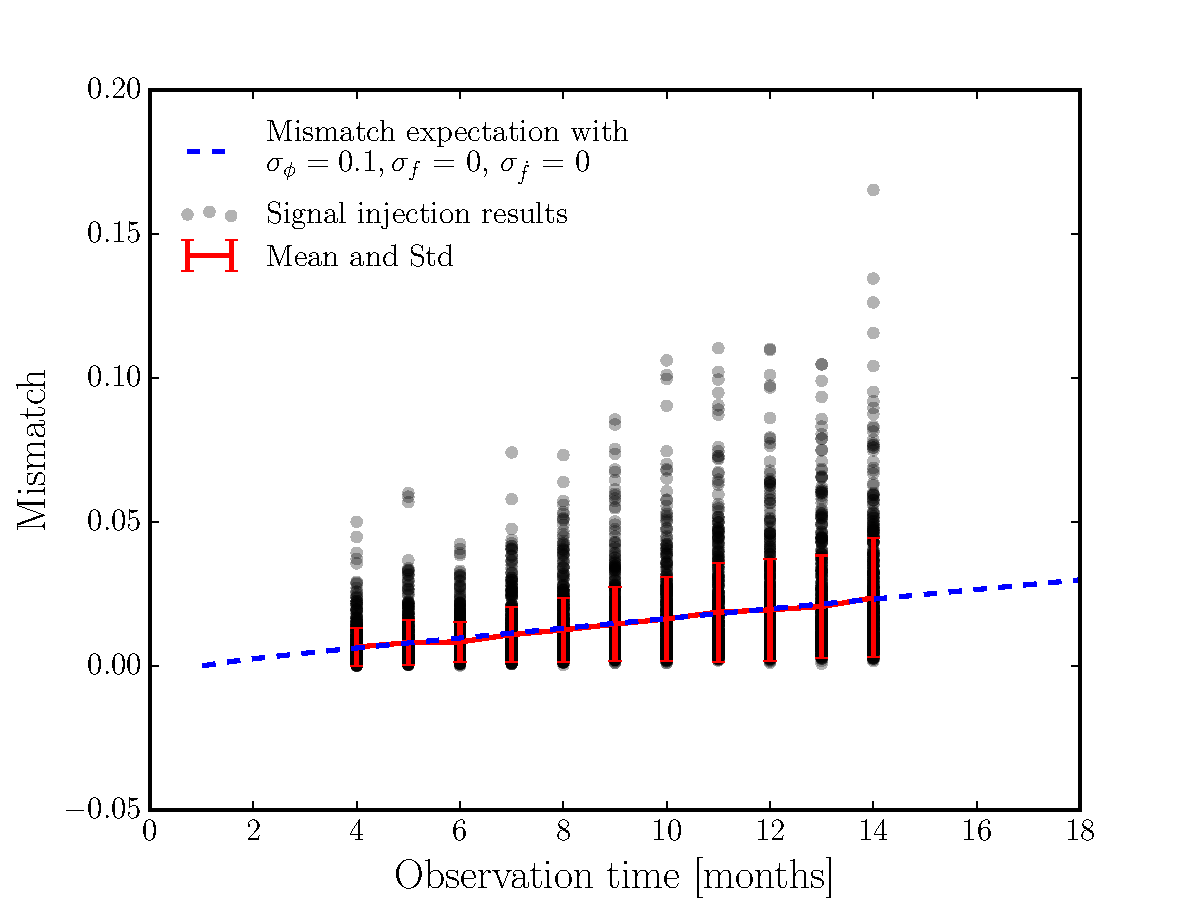
\includegraphics[width=0.5\textwidth]{ExpectationPhase}} 
\subfloat[Random walk in frequency]{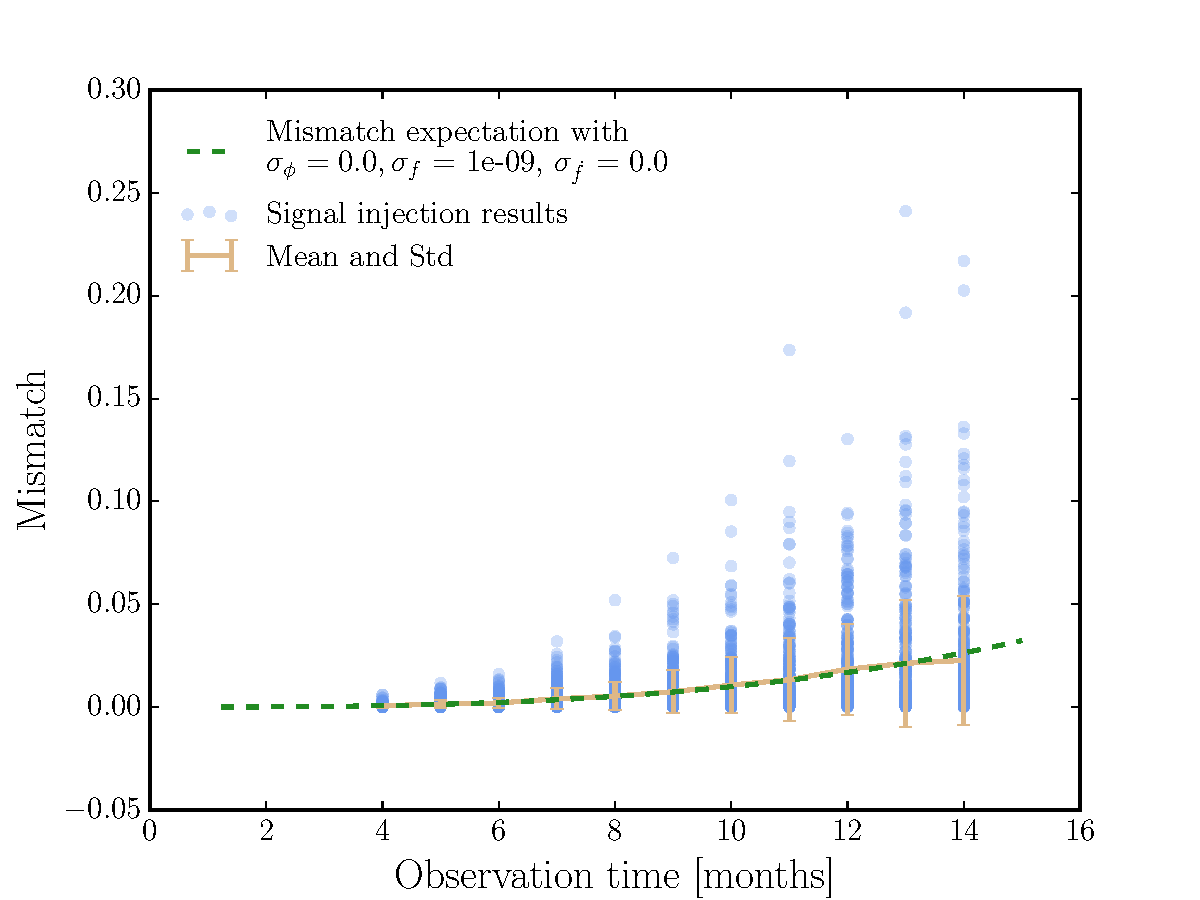
\includegraphics[width=0.5\textwidth]{ExpectationFrequency}}\\
\subfloat[Random walk in spin-down]{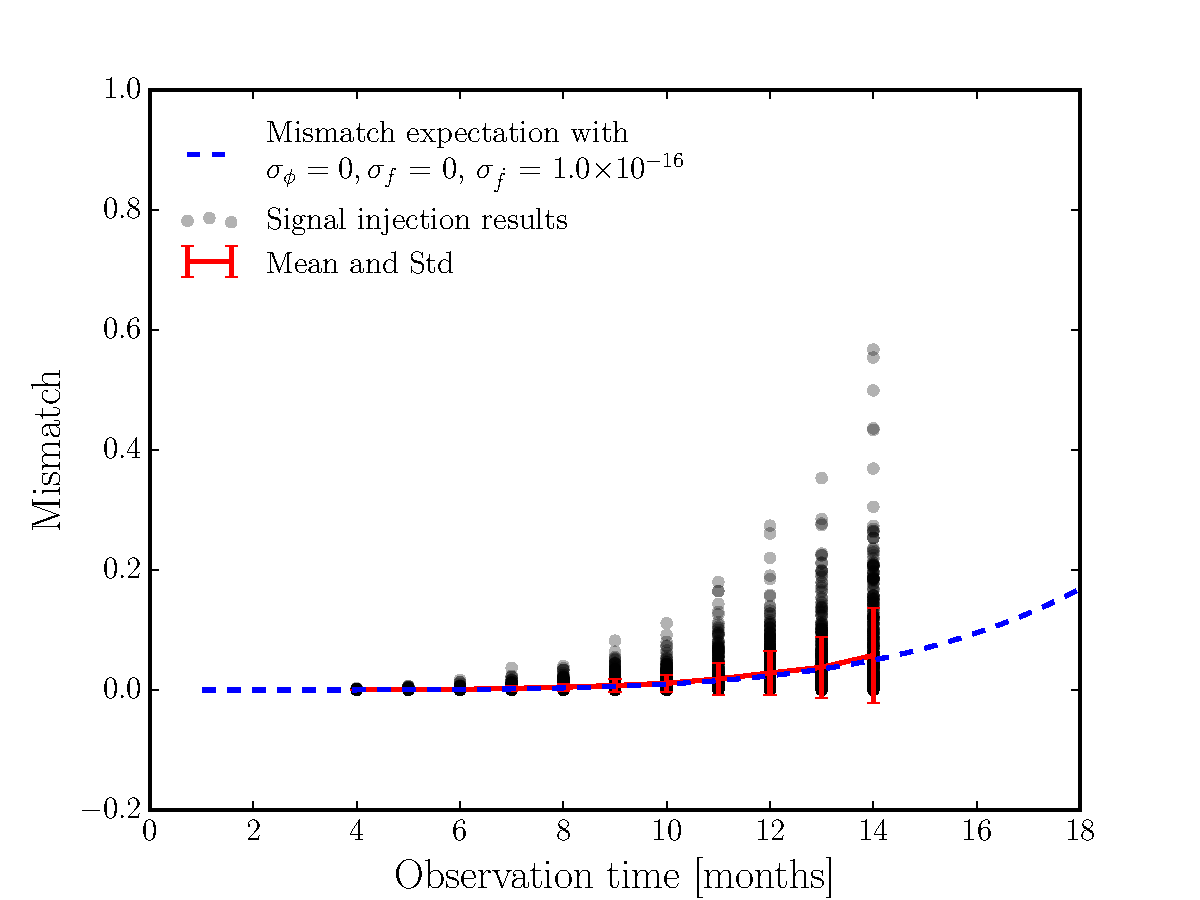
\includegraphics[width=0.5\textwidth]{ExpectationSpindown}}
\end{figure}•
\FloatBarrier

